{
This research, in accordance with the goals depicted in the previous section,
started by considering the collection of M stars provided by
DwarfArchives.org, a compendium of L, M and T dwarfs, 
maintained by Chris Gelino, Davy Kirkpatrick and Adam Burgasser.
}

\subsection{Dataset Selection.}
\label{subsec:DS}
{
The M dwarf database includes spectra for over 500 of the nearest and 
brightest M dwarfs in the same wavelength regime
(roughly 6300-9000{\AA} )(\cite{Kirkpatrick:2002eh}) with spectroscopic 
observations obtained at the Multiple Mirror Telescope (MMT, efective aperture 4.5m) 
on Mount Hopkins AZ and the McDonald Observatory 2.7 telescope on
Mount Locke, TX. The registered specrta from the IPAC dataset 
has no uncertainty defined.
}

{
At the MMT spectra were obtained with a Red Channel Spectrograph equipped 
with an 800x800 TI CCD. A 270 line mm\textsuperscript{-1} grating with an LP-945 order 
blocking filter was used to cover the range 6300 - 9000{\AA} at a resolution
of 18{\AA}. At McDonald, spectra covered the range 6400 - 9200{\AA} at a resolution 
of 12{\AA}(\cite{1994AJ....108.1437H}).
}

{
As the goal was to develop a procedure making possible to identify suitable 
reference bands for signal and continuum in this particular class of stars, 
it was decided to use synthetic spectra. We have choosed the library BT-Settl
(\cite{2013MSAIS..24..128A}) where several operations have been performed.
}

\subsection {Reshape of the theoretical library.}
\label{subsec:RTL}
{
Firstly a filterage looking for spectra between 2000 and 4200K was performed over 
the whole BT-Settl dataset, considering log(gravitiy) in range (-4, -6) dex 
with a step of 0.5 dex. Metallicity observed was between 0, -0.5 and -1 dex.

Spectra degradation from the original 0.1{\AA} stepsize till the required
according to the IPAC resolution (3.6{\AA}) was accomplished by a gaussian convolution
with 100 steps and a standard deviation of 3.6{\AA} too.
Then, the spectra are trimmed to produce valid segments between 6000 and 9150{\AA}.
}
{
Indeed, in order to become independent of the star\textquoteright s distance 
normalization the area under spectrum has been performed to value of one.
}
{
Total size of avaialble spectra is 429 (50K of distance each). 
As the total number of spectra is quite limited, we have decided to
interpollate between them, according to a finner parameter\textquoteright s mesh.
}

{
To be sure that interpolation was a valid solution to inferre new synthetic spectra,
a formal destillation of some spectra by using the 
PHOENIX code (\cite{fuhrmeister2005phoenix}) 
was performed and then, compared to the one obtained by interpollating in accordance 
to the inverse square of the distance among the closest neighborgs available 
(see Fig.~\ref{fig:comp_gen_inter}).
}

\begin {figure}
 \begin{center}
 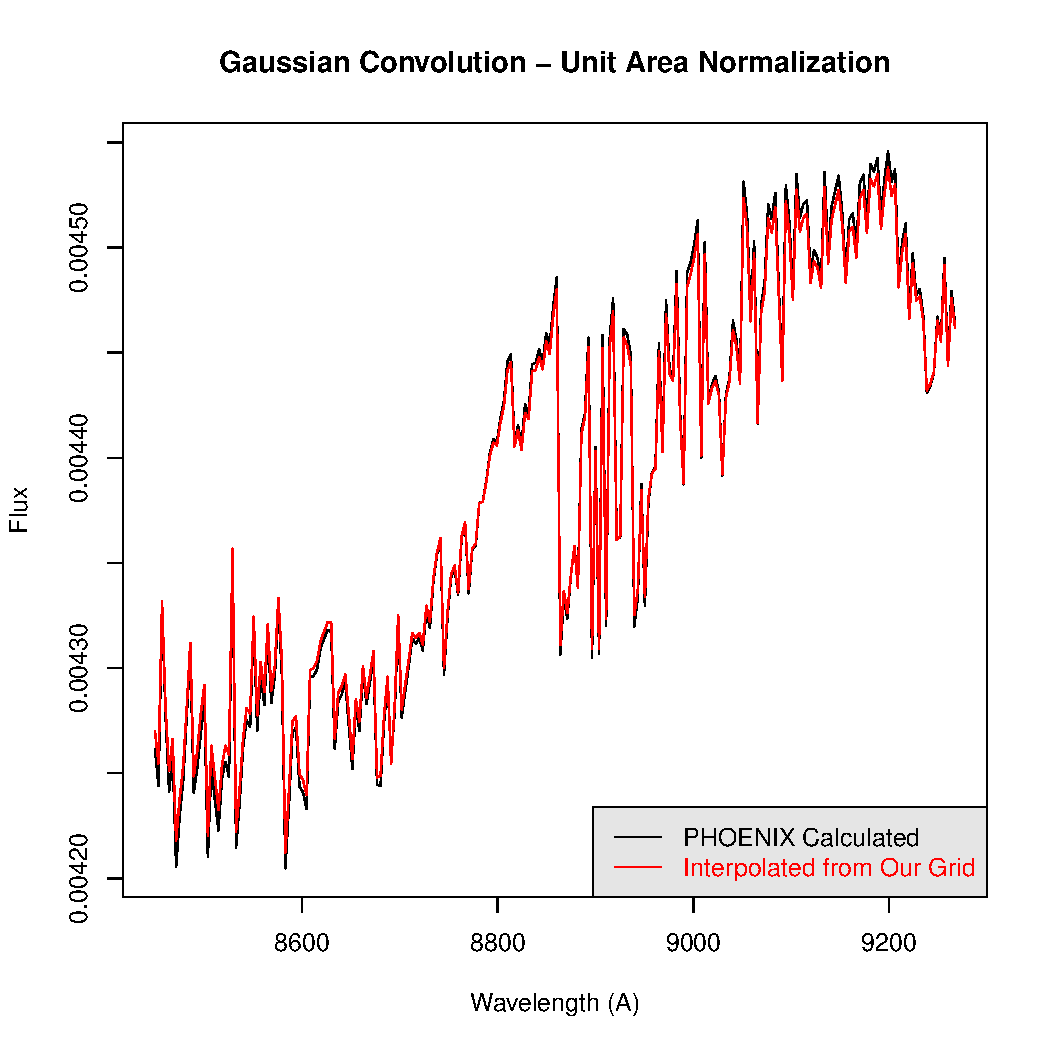
\includegraphics[width=6cm]{figs/intgrid4_gauss.pdf}
 \caption{Comparison between generated and interpollated spectrum}
 \label{fig:comp_gen_inter}
 \end{center}
\end {figure}

{
Now several other datasets have been created, by defininh a mesh of 0.25 dex for 
both, log(gravity) and Metallicity. Temperature step was selected to be 50K, 
which produced 1329 spectra.
Then, another reinterpolation is produced, with a new 
step for temperature of 25K and 0.125 dex for log(gravity), 
keeping the metallicity step in 0.25 dex and producing 
a dataset with 25912 spectra.
}

{
The synthetic spectra are theoretical and they are noise free but it 
does not happen with real spectra, the IPAC dataset in our case.
To increase similarities gaussian noise have been added with two 
different Signal to Noise Ratio(SNR). The selected SNR were 10 and 50.
}

\subsection{Feature definition}
\label{subsec:FD}
{
It is well known that due to the special characteristics of 
physical parameters for these stars it is not easy to define 
suitable signal bands but it is even more complicated to identify 
are the continuum chunks, were no signal shall be expected.
}

{
There are technical methodologies to identify suitable bands, as the one 
presented in (\cite{2013A&A...549A.129C}). %Cesetti ground base
In that case, bands I and K have been considered and prodosed and 
even when the dataset is a different one, the main 
band I (0.80 - 0.90${\mu}m$) is fully 
applicable in our research. Because of this their proposal for bands 
will be considered too in this research.
}

{
The underlying approach is to estimate the three star relevant physical 
parameters by establishing a set of features. These features consist of
a central bandpass covering the interesting lines and another bandpass
referring to the local continuum. Then, the feature can be written like 
Eq.~\eqref{eq:feature}.

\begin{equation}\label{eq:feature}
  F(i) =  \int_{\lambda_{1}(i)}^{\lambda_{2}(i)} \left( 1 - \frac{f(\lambda)}{F_{cont}(i)}\right) d{\lambda}  \quad \quad \forall i \in [1 \ldots N]
\end{equation}

and 

\begin{equation}\label{eq:cont}
 F_{cont}(i) =  \int_{\lambda_{1c}(i)}^{\lambda_{2c}(i)} f(\lambda) d{\lambda}   \quad \quad \forall i \in [1 \ldots N]
\end{equation}

where N means the number of features to be selected and $f(x)$ denotes the normalized spectra of the star in the 
region of interest.
}

{
Now, the research question is how to identify 
$\{\lambda_{1}(i),\lambda_{2}(i), \lambda_{1c}(i),\lambda_{2c}(i)\}  \quad \forall i \in [1 \ldots N] $
in such a way they become useful to estimate the physical parameters.
A few of minimal requirements need to be considered in the definition of those values like, for instance:

\begin{itemize}
 \item[$\diamond$]{ $ \lVert \lambda_{2}(i) - \lambda_{1}(i) \rVert  > 10 \AA \quad \forall i \in [1 \ldots N]$.}
 \item[$\diamond$]{ $ \lVert \lambda_{2c}(i) - \lambda_{1c}(i) \rVert  > 20 \AA \quad \forall i \in [1 \ldots N]$.} 
 \item[$\diamond$]{ $ \overline{\lambda_{2}(i)\lambda_{1}(i)}  \bigcap 
                      \overline{\lambda_{2c}(i)\lambda_{1c}(i)} = \emptyset \quad \forall i \in [1 \ldots N]$.}
\end{itemize}

which become a guarantee for avoiding any overlapping and a minimum size for both signal and continuum bandpasses.
}

\subsection{Determination of Features}
\label{subsec:DF}
{
To search for those features will depend on which specific phyisical parameter is 
under consideration but, the proposed methodology will look for those values 
trying to solve an optimization problem, which shall be the forecast capabilities
of one specific set of features, to be retained when it becomes bigger than 
a threshold.

To accomplish such optimization problem involving the selection of variable 
subsets, the use of the Genetic Algorithms technique was accepted. 
}

{
It was proposed to use the software tools R(\cite{R2013}).
There are different statistics to identify features 
that are differentially expressed between
two or more groups of samples and then uses the most differentially
expressed to construct a statistical model.
}

{
These methods have 
demonstrated to perform well, however, in some cases they can be ineffective
regardless of the classification method used. An obvious conceptual limitation
of univariate approaches is also the lack of consideration that features works in
the contexts of interconnected pathways and therefore it is their behaviour as
a group that may be predictive of the phenotypic variables. Multivariate
selection methods may seem to be more suitable for the analysis of 
data since variables are tested in
combination to identify interactions between features. However, the extremely
large number of models that can be constructed from different combination of
thousands of features cannot be extensively evaluated using standard
computational resources.
}

{
For the sake of simplicity let us define 
Genetic Algorithms (GAs) are variable search procedures that are based on
the principle of evolution by natural selection. The procedure works by
evolving sets of variables (chromosomes) that fit certain criteria from an initial
random population via cycles of differential replication, recombination and
mutation of the fittest chromosomes. The concept of using in-silico evolution
for the solution of optimization problems has been introduced by John
Holland in 1975 (\cite{holland1975adaptation}). Although their application has been
reasonably widespread (see Goldberg\textquoteright s 
book (\cite{goldberg1989genetic}), they became
very popular only when sufficiently powerful computers became available.
}

{
The implementation of the GA follows the next steps:
\begin{itemize}
 \item [\textbf{Stage 1}:]{To produce the population of potential features (chromosomes).}
 \item [\textbf{Stage 2}:]{Each chromosome in the population is evaluated for its ability to
predict the group membership of each sample in the dataset (fitness function).}
 \item [\textbf{Stage 3}:]{Chromosome preselection, when a chromosome has 
 a score higher then a predefined value.}
 \item [\textbf{Stage 4}:]{The population of chromosomes is replicated. 
 Chromosomes with a higher fitness score will 
 generate a more numerous offspring.}
 \item [\textbf{Stage 5}:]{The genetic information contained in the replicated parent
chromosomes is combined through genetic crossover. Two randomly selected
parent chromosomes are used to create two new chromosomes.}
 \item [\textbf{Stage 6}:]{Mutations are then introduced in the chromosome randomly. 
 These mutations produce that new genes are used in chromosomes.
 Steps 5 and 6 are applied over the chromosomes establised at Step 4.}
  \item [\textbf{Stage 7}:]{This process is repeated from Stage 2 until 
  enough accuracy is obtained or the maximum of iterations is attained.}
\end{itemize}

The four values for $\lambda$ required to define a 
gene were coded for working in \emph{band I} and 
they named according to the ordinal of the wavelength step.
A fixed number of genes where agreed as memeber per chromosome 
and we have used five for this pourpose.
}

{
The same strategy was used for all the three physical parameters $(T_{eff}, log(g), met)$.
As fitness function two of them were evalauted. The first one was the Nearest Center (\emph{NC}), 
defined as the point were the euclidean distance is minimum and it is a non
parametric method, thus it is not required the data follows a normal distribution.
The second one was the emsemble method known as Random Forest (\cite{breiman2001random}) (\emph{RF}), 
where fitness becomes the accuracy to predict the right classes for 
validation chromosomes. The RF fitness function is smarter but
the required computational effort is much higher than NC.
}

{
The fitness function uses the classification accuracy of the
model on the training samples to assign a score to each chromosome and
make possible the selection of better predictors through the law of natural
selection. There are different ways to estimate the error during training. The
most obvious one is to further split the training set into training and
validation sets.
}

{
The selected chromosomes have different persistence in population, but also
their rank is relevant in order to establish the notion of stability.
The Figure~\ref{fig:chr-stab} summarizes that concept as 
provided by package Galgo in library R.
\begin{figure}
\begin {center}
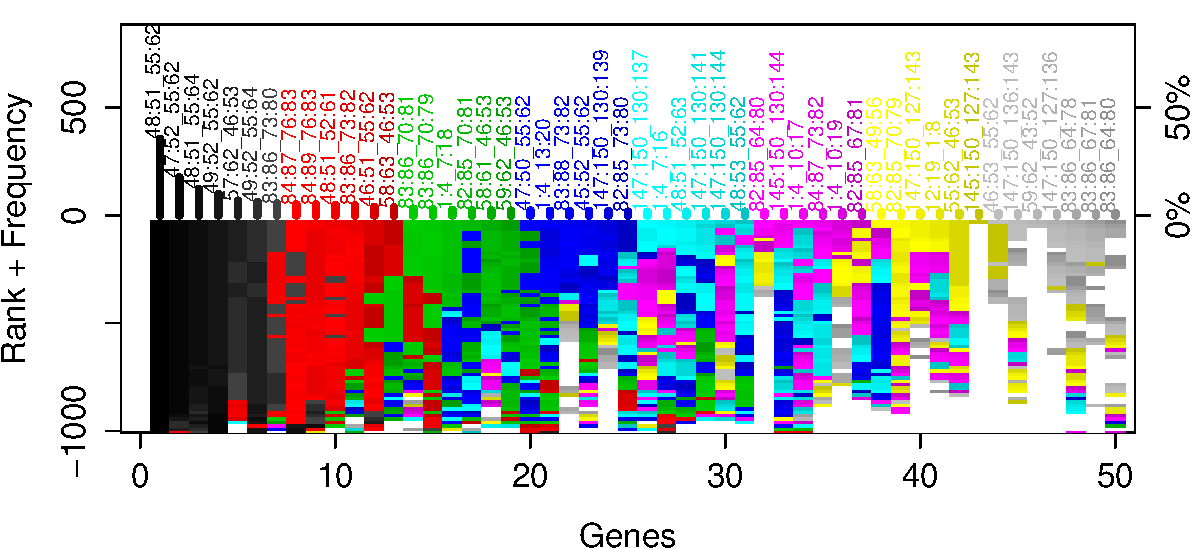
\includegraphics[width=10cm]{figs/ga_t_stab_crp.pdf}
\caption{Gene rank stability to predit $T_{eff}$ with a NC fitness fucntion}
\label{fig:chr-stab}
 \end{center}
\end{figure}

The most frequent fifty chromosomes were presented along the orizontal
axis in eight colors, with six or seven genes per color. Upper vertical
axis presents the gene frequency and the lower part of the vertical
axis describes the colour code for that gene in previous epochs.
This representation reflects both rank and persistence, wich can be seen 
as a metric for gene stability.
}

{
The GA procedure provides us with a large collection of chromosomes.
Although these are all good solutions of the problem, it is not clear which one
should be chosen for developing a model becoming for interpretation. 
For this reason there is a need to
develop a single model that is, to some extent, representative of the
population. The simpler strategy to follow is to use the frequency of genes in
the population of chromosomes as criteria for inclusion in a forward selection
strategy. The model of choice will be the one with the highest classification
accuracy and the lower number of genes.

After applying this technique the recommended features for temperature 
can be found in Table~\ref{tab:tab_NC_T}. 

\begin{table}
\begin{center}
\begin{tabular}{rrrrr}
  \hline
 & Signal\_from & Signal\_To & Cont\_From & Cont\_To \\ 
  \hline
Feature 1 & 8451.60 & 8458.80 & 8473.20 & 8509.20 \\ 
Feature 2 & 8620.80 & 8628.00 & 8646.00 & 8667.60 \\ 
Feature 3 & 8653.20 & 8667.60 & 8613.60 & 8635.20 \\ 
Feature 4 & 8746.80 & 8754.00 & 8710.80 & 8739.60 \\ 
Feature 5 & 8977.20 & 8984.40 & 8916.00 & 8937.60 \\ 
   \hline
\end{tabular}
\caption {Recommended features and Continuum bandpass for predicting $T_{eff}$ 
      by using NC fitness function} \label{tab:tab_NC_T} 
\end{center}
\end{table}

As in (\cite{2013A&A...549A.129C}) the authors provided their 
best estimation for suitable features, our interest is also to verify how
good it becomes in our particular case, as 
it can be an inderect assessment for the quality of the GA based recommendation. 
They have provided, inside the range of the IPAC dataset, the 
bandpass presented in Table~\ref{tab:tab_cesetti}

\begin{table}
\begin{center}
\begin{tabular}{rrrrrrr}
  \hline
 & Signal\_from & Signal\_To & Cont1\_From & Cont1\_To & Cont2\_From & Cont2\_To \\ 
  \hline
Pa1 & 8462.40 & 8473.20 & 8476.80 & 8484.00 & 8563.20 & 8574.00 \\ 
  Ca1 & 8484.00 & 8512.80 & 8476.80 & 8484.00 & 8563.20 & 8574.00 \\ 
  Ca2 & 8523.60 & 8559.60 & 8476.80 & 8484.00 & 8563.20 & 8574.00 \\ 
  Pa2 & 8577.60 & 8617.20 & 8563.20 & 8574.00 & 8620.80 & 8638.80 \\ 
  Ca3 & 8642.40 & 8682.00 & 8620.80 & 8638.80 & 8700.00 & 8721.60 \\ 
  Pa3 & 8732.40 & 8772.00 & 8700.00 & 8721.60 & 8779.20 & 8790.00 \\ 
  Mg & 8804.40 & 8808.00 & 8779.20 & 8790.00 & 8815.20 & 8847.60 \\ 
  Pa4 & 8851.20 & 8887.20 & 8815.20 & 8847.60 & 8890.80 & 8898.00 \\ 
   \hline
\end{tabular}
\caption {Recommended features and Continuum bandpass recommended in 
   \cite{2013A&A...549A.129C} as relevant for temperature}
   \label{tab:tab_cesetti} 
\end{center}
\end{table}

In regards with the Gravity, the GA recommends the features 
presentend in Table~\ref{tab:tab_NC_G}

\begin{table}
\begin{center}
\begin{tabular}{rrrrr}
  \hline
 & Signal\_from & Signal\_To & Cont\_From & Cont\_To \\ 
  \hline
Feature 1 & 8462.40 & 8476.80 & 8484.00 & 8520.00 \\ 
Feature 2 & 8620.80 & 8628.00 & 8667.60 & 8703.60 \\ 
Feature 3 & 8646.00 & 8653.20 & 8689.20 & 8710.80 \\ 
Feature 4 & 8656.80 & 8664.00 & 8689.20 & 8718.00 \\ 
Feature 5 & 8782.80 & 8790.00 & 8797.20 & 8818.80 \\ 
   \hline
\end{tabular}
\caption {Recommended features and Continuum bandpass for predicting $log(g)$ 
      by using NC fitness function} \label{tab:tab_NC_G} 
\end{center}
\end{table}

Finally, features suggested for metallicity 
can be found in Table~\ref{tab:tab_NC_M}.

\begin{table}
\begin{center}
\begin{tabular}{rrrrr}
  \hline
 & Signal\_from & Signal\_To & Cont\_From & Cont\_To \\ 
  \hline
Feature 1 & 8516.40 & 8538.00 & 8548.80 & 8577.60 \\ 
Feature 2 & 8620.80 & 8628.00 & 8635.20 & 8671.20 \\ 
Feature 3 & 8782.80 & 8790.00 & 8797.20 & 8818.80 \\ 
Feature 4 & 8970.00 & 8977.20 & 8916.00 & 8952.00 \\ 
Feature 5 & 9009.60 & 9016.80 & 8980.80 & 9002.40 \\ 
   \hline
\end{tabular}
\caption {Recommended features and Continuum bandpass for predicting $Metallicity$ 
      by using NC fitness function} \label{tab:tab_NC_M} 
\end{center}
\end{table}


}